% !TEX root = ../main.tex
% 本文件由 build-tex.sh 从 18-DSP指南-第18章中译.md 生成，改内容请改 md 后重新生成

\chapter{FFT 卷积}\label{ch-18}

本章介绍两种重要的 DSP 技术：重叠相加法(overlap-add method)和 FFT
卷积(FFT convolution)。重叠相加法用来把长信号切成较短的段，以便处理。FFT
卷积把重叠相加法和快速傅里叶变换（Fast Fourier
Transform，FFT）结合起来，通过把两个信号的频谱相乘来完成卷积。对于长度超过大约
64 点的滤波器核，FFT 卷积比标准卷积更快，而结果完全相同。

\section{重叠相加法}

在许多 DSP 应用中，长信号必须分段滤波。例如，高保真数字音频的数据率约为
5 MB/分钟，数字视频约为 500
MB/分钟。数据率这么高，计算机的内存常常不够同时容纳要处理的整个信号。还有一些系统因为是实时运行的，只能一段一段地处理。例如，电话信号的延迟不能超过几百毫秒，这就限制了任何时刻能拿来处理的数据量。还有一些应用，是处理方法本身要求把信号分段。FFT
卷积就是一个例子，它也是本章的主题。

重叠相加法基于 DSP 的基本技巧：(1) 把信号分解成简单的分量；(2)
以某种有用的方式处理每个分量；(3) 把处理过的分量重新合成最终的信号。图
18-1 展示了重叠相加法怎样做到这一点。图 (a) 是要滤波的信号，(b)
是要用的滤波器核，一个窗函数 sinc 低通滤波器(windowed-sinc low-pass
filter)。跳到图的最下面，(i) 是滤波后的信号，是 (a)
的平滑版本。这种方法的关键在于卷积怎样影响这些信号的长度。一个 N
点信号与一个 M 点滤波器核卷积，输出信号长 N + M − 1 点。例如，输入信号
(a) 有 300 个采样（从 0 到 299），滤波器核 (b) 有 101 个采样（从 0 到
100），输出信号 (i) 有 400 个采样（从 0 到 399）。

换句话说，一个 N 点信号经过滤波后，会向右扩展 M − 1
个点。（这里假定滤波器核的下标从 0
开始。如果滤波器核用了负下标，信号也会向左扩展。）在 (a) 中，第 300 到
399 个采样处补上了零，用来表示扩展会发生在哪里。别被输出信号 (i)
两端那些很小的值迷惑了，这只是因为窗函数 sinc 滤波器核两端的值很小。(i)
中的全部 400 个采样都不为零，只是有些小到在图上看不出来。

图 (c)、(d)、(e)
展示了重叠相加法所用的分解。信号被切成若干段，每段包含原信号的 100
个采样。此外，每段右边再补上 100
个零。下一步，把每段分别与滤波器核卷积，单独滤波。这样就得到
(f)、(g)、(h) 所示的输出段。由于每个输入段长 100 个采样、滤波器核长 101
个采样，每个输出段将长 200 个采样。要理解的重点是：每个输入段补上 100
个零，就是为了给卷积时的扩展留出位置。

注意，扩展使得各输出段彼此重叠。把这些重叠的输出段相加，就得到输出信号
(i)。例如，(i) 中第 200 到 299 个采样，是把 (g) 和 (h)
中对应的采样相加得到的。重叠相加法得到的输出信号与直接卷积完全相同。缺点是程序要复杂得多，因为必须记录哪些采样是重叠的。

\begin{figure}[htbp]
\centering
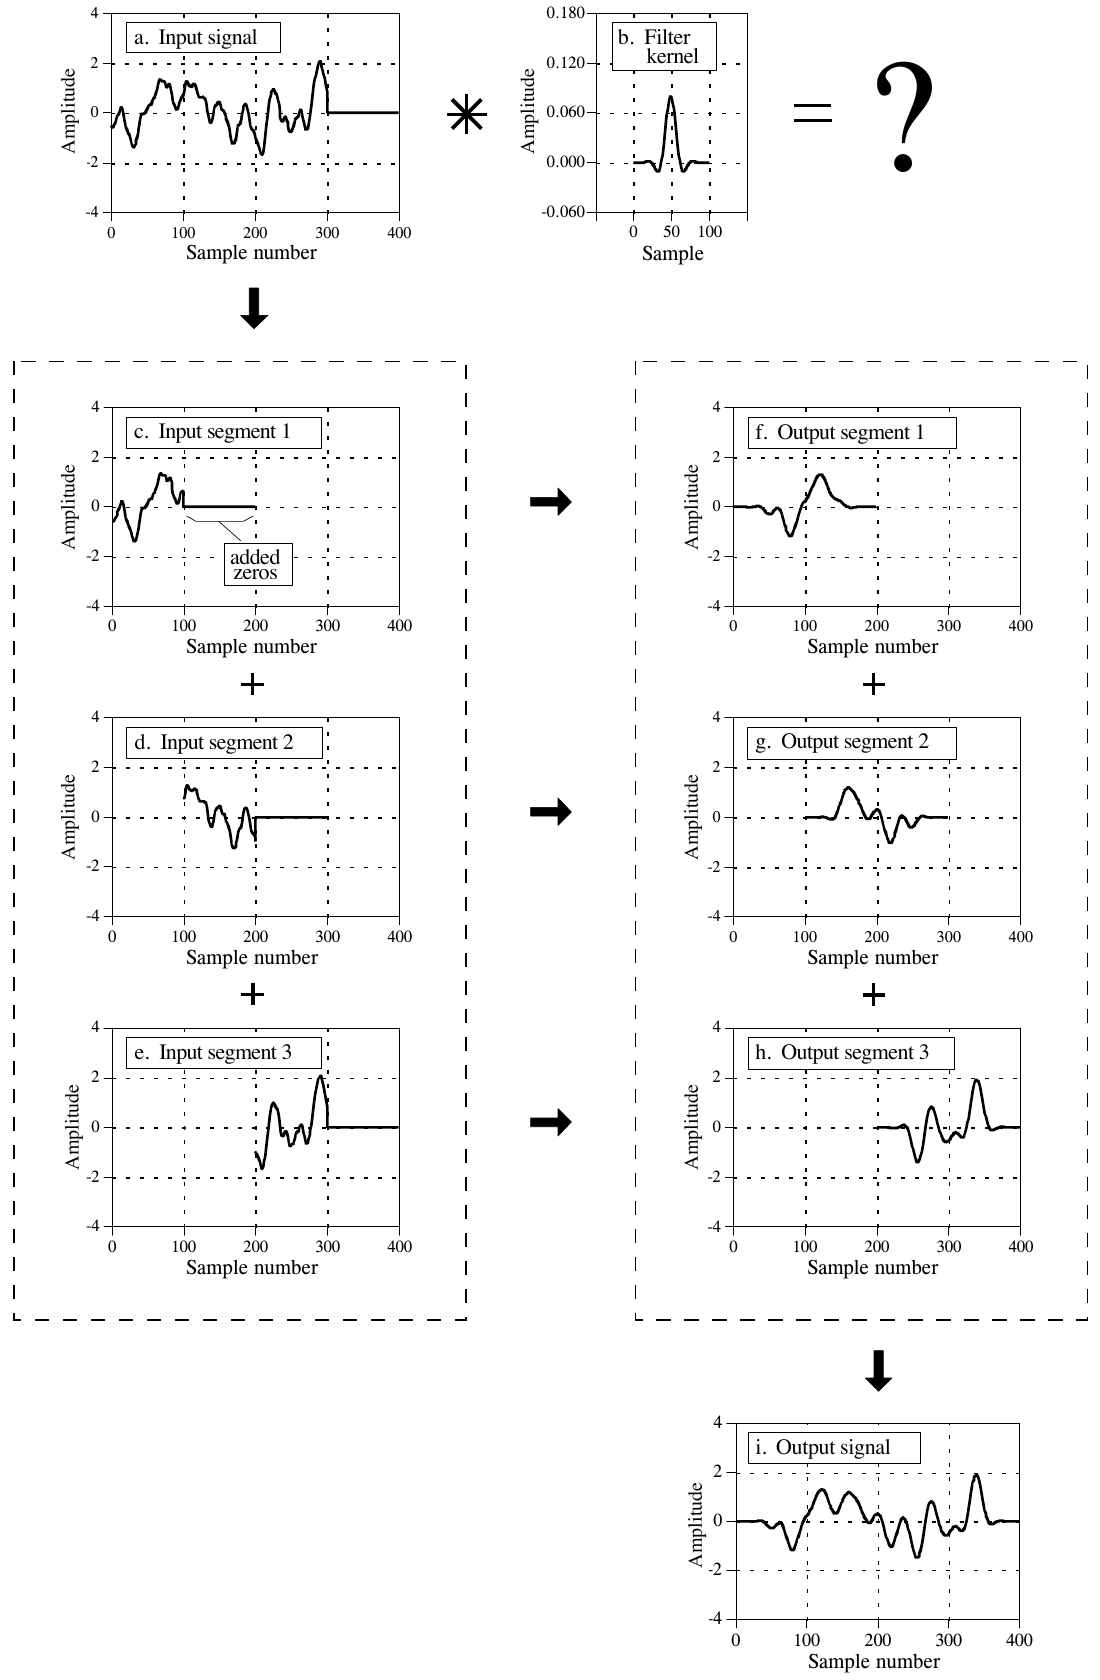
\includegraphics[width=0.917\linewidth,height=0.8\textheight,keepaspectratio]{assets/ch18/fig18-01.png}
\caption*{\textbf{图 18-1　重叠相加法。} 目标是把输入信号 (a) 与滤波器核 (b)
卷积。做法是把输入信号切成若干段，比如
(c)、(d)、(e)，每段补上足够多的零，为卷积时的扩展留出位置。把每个输入段与滤波器核卷积，得到输出段
(f)、(g)、(h)。再把这些重叠的输出段相加，就得到输出信号 (i)。 （a. Input
signal = 输入信号；b. Filter kernel = 滤波器核；c～e. Input segment 1～3
= 输入段 1～3，added zeros = 补上的零；f～h. Output segment 1～3 =
输出段 1～3；i. Output signal = 输出信号。Amplitude = 幅度，Sample
number / Sample = 采样序号。第一行的 \dspsym{∗} 是卷积。原书图注排在 (i)
的左边，裁图时已去掉，译文见上。）}
\end{figure}

\section{FFT 卷积}

FFT 卷积利用的原理是：频域中的乘法对应时域中的卷积。先用 DFT
把输入信号变换到频域，乘以滤波器的频率响应，再用逆 DFT
变换回时域。这个基本技术从傅里叶的年代就已为人所知，但当时没有人真正在意。原因是计算
DFT 所需的时间，比直接计算卷积的时间还长。1965
年快速傅里叶变换（FFT）的出现改变了这一点。用 FFT 算法来计算
DFT，经由频域的卷积就能比直接在时域卷积更快。最终结果是一样的，只是更高效的算法改变了计算量。因此，FFT
卷积也叫高速卷积(high-speed convolution)。

FFT 卷积使用图 18-1
所示的重叠相加法，改变的只是把输入段变成输出段的方式。图 18-2 展示了 FFT
卷积怎样把一个输入段变成一个输出段。首先，用 FFT 对滤波器核做
DFT，求出滤波器的频率响应。例如，(a) 是一个示例滤波器核，一个窗函数 sinc
带通滤波器(band-pass filter)。FFT 把它变成频率响应的实部和虚部，见 (b)
和
(c)。这些频域信号可能看起来不像带通滤波器，因为它们是直角坐标形式。记住，人理解频域通常用极坐标形式最好，而数学计算通常用直角坐标形式最好。这些实部和虚部存放在计算机里，留待计算每一段时使用。

图 (d) 是正在处理的输入段。用 FFT 求出它的频谱，见 (e) 和
(f)。然后把滤波器的频率响应 (b)、(c) 乘以输入段的频谱
(e)、(f)，得到输出段的频谱
(h)、(i)。由于这些频谱由实部和虚部组成，要按第 9 章的公式 9-1
相乘。再用逆 FFT 从频谱 (h)、(i) 求出输出段
(g)。重要的是要认识到，这个输出段与把输入段 (d) 和滤波器核 (a)
直接卷积得到的结果完全相同。

FFT 必须足够长，才不会发生循环卷积(circular convolution)（第 9
章也讲过）。这意味着 FFT 的长度应当与输出段 (g) 的长度相同。例如，在图
18-2 的例子中，滤波器核有 129 点，每段有 128 点，所以输出段长 256
点。这就要求使用 256 点 FFT。也就是说，滤波器核 (a) 必须补上 127
个零，使总长度达到 256 点。同样，每个输入段 (d) 必须补上 128
个零。再举一个例子，设想你要把一个很长的信号与一个 600
点的滤波器核卷积。一种选择是每段 425 点、用 1024 点
FFT；另一种选择是每段 1449 点、用 2048 点 FFT。

\begin{figure}[htbp]
\centering
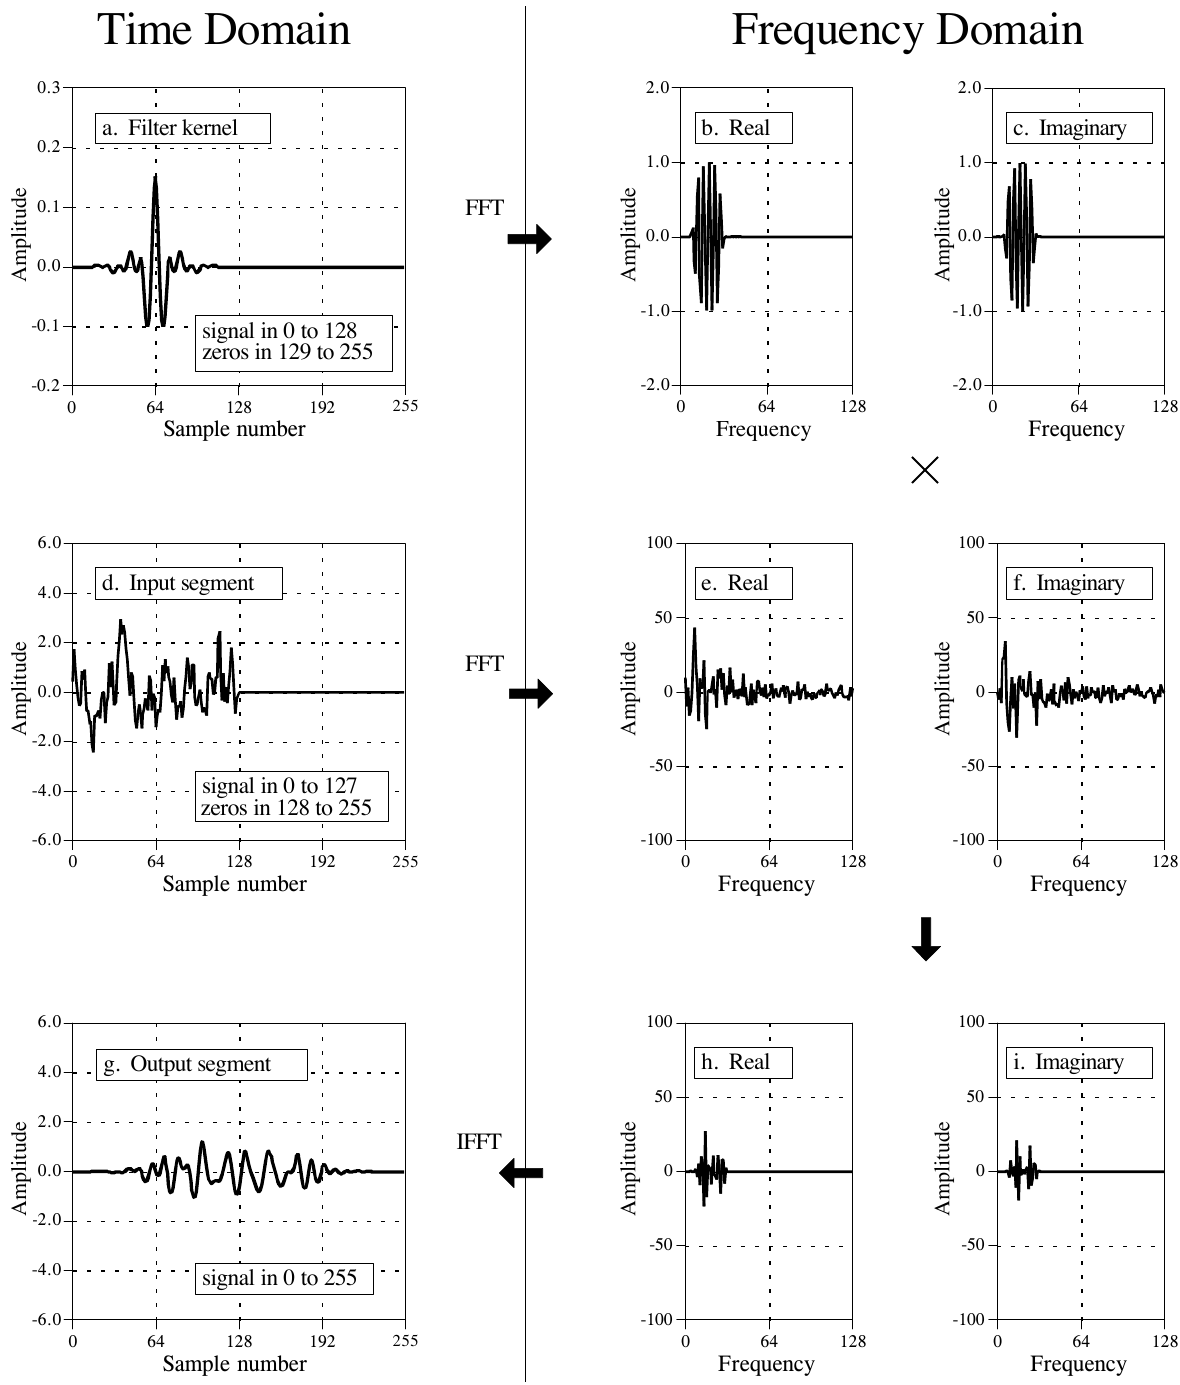
\includegraphics[width=0.983\linewidth,height=0.8\textheight,keepaspectratio]{assets/ch18/fig18-02.png}
\caption*{\textbf{图 18-2　FFT 卷积。} 滤波器核 (a) 和信号段 (d) 经 FFT
分别变成各自的频谱 (b)、(c) 和
(e)、(f)。这两个频谱相乘，得到输出段的频谱 (h)、(i)。再由逆 FFT
求出输出段 (g)。 （Time Domain = 时域，Frequency Domain = 频域；a.
Filter kernel = 滤波器核，signal in 0 to 128, zeros in 129 to 255 = 第
0～128 点是信号，第 129～255 点是零；b/e/h. Real = 实部；c/f/i.
Imaginary = 虚部；d.~Input segment = 输入段，signal in 0 to 127, zeros
in 128 to 255 = 第 0～127 点是信号，第 128～255 点是零；g. Output
segment = 输出段，signal in 0 to 255 = 第 0～255 点都是信号。FFT
箭头表示正变换，IFFT 表示逆变换，× 表示两个频谱相乘。Amplitude =
幅度，Sample number = 采样序号，Frequency =
频率。原书图注把输入段的频谱写成 ``(d) \& (e)''，应为 (e) 和
(f)，译文已改正。）}
\end{figure}

表 18-1 是一个执行 FFT 卷积的示例程序。这个程序把一个 1000
万点的信号与一个 400 点的滤波器核卷积。做法是把输入信号切成 16000
段，每段 625 点。每段与滤波器核卷积，得到一个 625 + 400 − 1 = 1024
点的输出段。因此使用 1024 点 FFT。在定义并初始化所有数组之后（第
130～230 行），第一步是计算并保存滤波器的频率响应（第 250～310 行）。第
260 行调用一个虚构的子程序，把滤波器核载入 XX{[}0{]} 到
XX{[}399{]}，并把 XX{[}400{]} 到 XX{[}1023{]} 设为零。第 270
行的子程序是 FFT，把 XX{[} {]} 中的 1024 个采样变换成 REX{[} {]} 和
IMX{[} {]} 中的 513 个采样，即频率响应的实部和虚部。这些值被转存到数组
REFR{[} {]} 和 IMFR{[} {]} 中（意为 REal and IMaginary Frequency
Response，频率响应的实部和虚部），供程序后面使用。

第 340 到 580 行之间的 FOR-NEXT 循环控制 16000 段的处理。在第 360
行，一个子程序把下一段要处理的数据载入 XX{[}0{]} 到 XX{[}624{]}，并把
XX{[}625{]} 到 XX{[}1023{]} 设为零。在第 370 行，用 FFT
子程序求出这一段的频谱，实部放进 REX{[} {]} 的 513 个点，虚部放进 IMX{[}
{]} 的 513 个点。第 390～430 行是把这一段的频谱（存放在 REX{[} {]} 和
IMX{[} {]}）乘以滤波器的频率响应（存放在 REFR{[} {]} 和 IMFR{[}
{]}）。相乘的结果存回 REX{[} {]} 和 IMX{[}
{]}，覆盖原来的数据。由于这时它已经是输出段的频谱，就可以用 IFFT
求出输出段。这由第 450 行虚构的 IFFT 子程序完成，它把 REX{[} {]} 和
IMX{[} {]} 中的 513 个点变换成 XX{[} {]} 中的 1024 个点，即输出段。

第 470～550 行处理段与段之间的重叠。每个输出段分为两部分。前 625 个点（0
到 624）需要与上一个输出段的重叠部分相加，然后写入输出信号。后 399
个点（625 到 1023）需要保存起来，以便与下一个输出段重叠。

要理解这一点，回头看图 18-1。(g) 中第 100 到 199
个采样需要与上一个输出段 (f) 的重叠部分相加，然后就可以移到输出信号 (i)
中。相比之下，(g) 中第 200 到 299 个采样需要保存起来，以便与下一个输出段
(h) 相加。

现在回到程序。数组 OLAP{[} {]} 用来存放从一段重叠到下一段的 399
个采样。在第 470～490 行，把这个数组中（来自上一个输出段）的 399
个值加到当前正在处理的输出段上，该输出段存放在 XX{[} {]} 中。然后第 550
行的虚构子程序把 XX{[}0{]} 到 XX{[}624{]} 中的 625
个采样输出到存放输出信号的文件。当前输出段中需要留给下一个输出段的 399
个采样，在第 510～530 行存入 OLAP{[} {]}。

第 0 到 15999 段全部处理完后，数组 OLAP{[} {]} 中存放的是第 15999
段中应当与第 16000 段重叠的 399 个采样。由于第 16000
段并不存在（或者可以看作全是零），这 399 个采样在第 600
行直接写入输出信号。这使得输出信号的长度为 16000 × 625 + 399 =
10,000,399 点。这正好等于输入信号的长度加上滤波器核的长度再减一。

\textbf{表 18-1}（注释已译成中文）

\begin{Shaded}
\begin{Highlighting}[]
\NormalTok{100 \textquotesingle{}FFT 卷积}
\NormalTok{110 \textquotesingle{}本程序把一个 1000 万点的信号与一个 400 点的滤波器核卷积。输入}
\NormalTok{120 \textquotesingle{}信号切成 16000 段，每段 625 点。使用 1024 点 FFT。}
\NormalTok{130 \textquotesingle{}}
\NormalTok{130 \textquotesingle{}                                \textquotesingle{}初始化各数组}
\NormalTok{140 DIM XX[1023]                     \textquotesingle{}时域信号（供 FFT 使用）}
\NormalTok{150 DIM REX[512]                     \textquotesingle{}频域的实部（供 FFT 使用）}
\NormalTok{160 DIM IMX[512]                     \textquotesingle{}频域的虚部（供 FFT 使用）}
\NormalTok{170 DIM REFR[512]                    \textquotesingle{}滤波器频率响应的实部}
\NormalTok{180 DIM IMFR[512]                    \textquotesingle{}滤波器频率响应的虚部}
\NormalTok{190 DIM OLAP[398]                    \textquotesingle{}存放段与段之间重叠的采样}
\NormalTok{200 \textquotesingle{}}
\NormalTok{210 FOR I\% = 0 TO 398                \textquotesingle{}把存放重叠采样的数组清零}
\NormalTok{220 OLAP[I\%] = 0}
\NormalTok{230 NEXT I\%}
\NormalTok{240 \textquotesingle{}}
\NormalTok{250 \textquotesingle{}                                \textquotesingle{}求出并保存滤波器的频率响应}
\NormalTok{260 GOSUB XXXX                       \textquotesingle{}虚构的子程序，把滤波器核载入 XX[ ]}
\NormalTok{270 GOSUB XXXX                       \textquotesingle{}虚构的 FFT 子程序：XX[ ] {-}{-}\textgreater{} REX[ ] \& IMX[ ]}
\NormalTok{280 FOR F\% = 0 TO 512                \textquotesingle{}把频率响应存入 REFR[ ] 和 IMFR[ ]}
\NormalTok{290 REFR[F\%] = REX[F\%]}
\NormalTok{300 IMFR[F\%] = IMX[F\%]}
\NormalTok{310 NEXT F\%}
\NormalTok{320 \textquotesingle{}}
\NormalTok{330 \textquotesingle{}                                \textquotesingle{}逐个处理 16000 段}
\NormalTok{340 FOR SEGMENT\% = 0 TO 15999}
\NormalTok{350 \textquotesingle{}}
\NormalTok{360 GOSUB XXXX                       \textquotesingle{}虚构的子程序，把下一个输入段载入 XX[ ]}
\NormalTok{370 GOSUB XXXX                       \textquotesingle{}虚构的 FFT 子程序：XX[ ] {-}{-}\textgreater{} REX[ ] \& IMX[ ]}
\NormalTok{380 \textquotesingle{}}
\NormalTok{390 FOR F\% = 0 TO 512                \textquotesingle{}频谱乘以频率响应}
\NormalTok{400 TEMP    = REX[F\%]*REFR[F\%] {-} IMX[F\%]*IMFR[F\%]}
\NormalTok{410 IMX[F\%] = REX[F\%]*IMFR[F\%] + IMX[F\%]*REFR[F\%]}
\NormalTok{420 REX[F\%] = TEMP}
\NormalTok{430 NEXT F\%}
\NormalTok{440 \textquotesingle{}}
\NormalTok{450 GOSUB XXXX                       \textquotesingle{}虚构的 IFFT 子程序：REX[ ] \& IMX[ ] {-}{-}\textgreater{} XX[ ]}
\NormalTok{460 \textquotesingle{}}
\NormalTok{470 FOR I\% = 0 TO 398                \textquotesingle{}把上一段的重叠部分加到这一段上}
\NormalTok{480 XX[I\%] = XX[I\%] + OLAP[I\%]}
\NormalTok{490 NEXT I\%}
\NormalTok{500 \textquotesingle{}}
\NormalTok{510 FOR I\% = 625 TO 1023             \textquotesingle{}保存要与下一段重叠的采样}
\NormalTok{520 OLAP[I\%{-}625] = XX[I\%]}
\NormalTok{530 NEXT I\%}
\NormalTok{540 \textquotesingle{}}
\NormalTok{550 GOSUB XXXX                       \textquotesingle{}虚构的子程序，输出存放在}
\NormalTok{560 \textquotesingle{}                                \textquotesingle{}XX[0] 到 XX[624] 中的 625 个采样}
\NormalTok{570 \textquotesingle{}}
\NormalTok{580 NEXT SEGMENT\%}
\NormalTok{590 \textquotesingle{}}
\NormalTok{600 GOSUB XXXX                       \textquotesingle{}虚构的子程序，输出 OLAP[ ] 中的全部 399 个采样}
\NormalTok{610 END}
\end{Highlighting}
\end{Shaded}

\begin{quote}
\textbf{译注：} 原书第 130 行重复出现了两次，是排版错误，不影响理解。
\end{quote}

\textbf{C 实现}（完整可编译版本见
\texttt{c/table18-1\_fft\_convolution.c}。原书的 FFT、IFFT
和数据读写都是''虚构的子程序''，这里 FFT 用表 12-4 的复数 FFT，逆 FFT
用表 12-5 的共轭法；为了能和直接卷积逐点对比，默认只处理 160
段，段数可用命令行参数修改）：

\begin{Shaded}
\begin{Highlighting}[]
\PreprocessorTok{\#define NFFT }\DecValTok{1024}\PreprocessorTok{                           }\CommentTok{/* 140 DIM XX[1023]：FFT 长度 */}
\PreprocessorTok{\#define NSEG }\DecValTok{625}\PreprocessorTok{                            }\CommentTok{/* 每段输入的点数 */}
\PreprocessorTok{\#define NK   }\DecValTok{400}\PreprocessorTok{                            }\CommentTok{/* 滤波器核的点数 */}
\PreprocessorTok{\#define NOL  }\OperatorTok{(}\PreprocessorTok{NK }\OperatorTok{{-}}\PreprocessorTok{ }\DecValTok{1}\OperatorTok{)}\PreprocessorTok{                       }\CommentTok{/* 190 DIM OLAP[398]：段与段之间重叠的 399 点 */}

\CommentTok{/* FFT 卷积主体，对应原书第 210～600 行。x 长 nseg*NSEG，y 长 nseg*NSEG + NOL */}
\DataTypeTok{static} \DataTypeTok{void}\NormalTok{ fft\_convolve}\OperatorTok{(}\DataTypeTok{const} \DataTypeTok{double} \OperatorTok{*}\NormalTok{x}\OperatorTok{,} \DataTypeTok{const} \DataTypeTok{double} \OperatorTok{*}\NormalTok{h}\OperatorTok{,} \DataTypeTok{int}\NormalTok{ nseg}\OperatorTok{,} \DataTypeTok{double} \OperatorTok{*}\NormalTok{y}\OperatorTok{)}
\OperatorTok{\{}
    \DataTypeTok{static} \DataTypeTok{double}\NormalTok{ xx}\OperatorTok{[}\NormalTok{NFFT}\OperatorTok{],}\NormalTok{ imx}\OperatorTok{[}\NormalTok{NFFT}\OperatorTok{];}          \CommentTok{/* 140～160：XX[ ]、REX[ ]（与 XX 共用）、IMX[ ] */}
    \DataTypeTok{static} \DataTypeTok{double}\NormalTok{ refr}\OperatorTok{[}\NormalTok{NFFT}\OperatorTok{],}\NormalTok{ imfr}\OperatorTok{[}\NormalTok{NFFT}\OperatorTok{];}       \CommentTok{/* 170～180：滤波器的频率响应 */}
    \DataTypeTok{double}\NormalTok{ olap}\OperatorTok{[}\NormalTok{NOL}\OperatorTok{];}                           \CommentTok{/* 190 */}

    \ControlFlowTok{for} \OperatorTok{(}\DataTypeTok{int}\NormalTok{ i }\OperatorTok{=} \DecValTok{0}\OperatorTok{;}\NormalTok{ i }\OperatorTok{\textless{}}\NormalTok{ NOL}\OperatorTok{;}\NormalTok{ i}\OperatorTok{++)}\NormalTok{ olap}\OperatorTok{[}\NormalTok{i}\OperatorTok{]} \OperatorTok{=} \DecValTok{0}\OperatorTok{;}  \CommentTok{/* 210～230：重叠数组清零 */}

    \ControlFlowTok{for} \OperatorTok{(}\DataTypeTok{int}\NormalTok{ i }\OperatorTok{=} \DecValTok{0}\OperatorTok{;}\NormalTok{ i }\OperatorTok{\textless{}}\NormalTok{ NFFT}\OperatorTok{;}\NormalTok{ i}\OperatorTok{++)} \OperatorTok{\{}            \CommentTok{/* 260：核放进 XX[0]～XX[399]，其余补零 */}
\NormalTok{        refr}\OperatorTok{[}\NormalTok{i}\OperatorTok{]} \OperatorTok{=}\NormalTok{ i }\OperatorTok{\textless{}}\NormalTok{ NK }\OperatorTok{?}\NormalTok{ h}\OperatorTok{[}\NormalTok{i}\OperatorTok{]} \OperatorTok{:} \FloatTok{0.0}\OperatorTok{;}
\NormalTok{        imfr}\OperatorTok{[}\NormalTok{i}\OperatorTok{]} \OperatorTok{=} \FloatTok{0.0}\OperatorTok{;}
    \OperatorTok{\}}
\NormalTok{    fft}\OperatorTok{(}\NormalTok{refr}\OperatorTok{,}\NormalTok{ imfr}\OperatorTok{,}\NormalTok{ NFFT}\OperatorTok{);}                      \CommentTok{/* 270～310：求出并保存滤波器的频率响应 */}

    \ControlFlowTok{for} \OperatorTok{(}\DataTypeTok{int}\NormalTok{ seg }\OperatorTok{=} \DecValTok{0}\OperatorTok{;}\NormalTok{ seg }\OperatorTok{\textless{}}\NormalTok{ nseg}\OperatorTok{;}\NormalTok{ seg}\OperatorTok{++)} \OperatorTok{\{}      \CommentTok{/* 340：逐段处理 */}
        \ControlFlowTok{for} \OperatorTok{(}\DataTypeTok{int}\NormalTok{ i }\OperatorTok{=} \DecValTok{0}\OperatorTok{;}\NormalTok{ i }\OperatorTok{\textless{}}\NormalTok{ NFFT}\OperatorTok{;}\NormalTok{ i}\OperatorTok{++)} \OperatorTok{\{}        \CommentTok{/* 360：本段放进 XX[0]～XX[624]，其余补零 */}
\NormalTok{            xx}\OperatorTok{[}\NormalTok{i}\OperatorTok{]} \OperatorTok{=}\NormalTok{ i }\OperatorTok{\textless{}}\NormalTok{ NSEG }\OperatorTok{?}\NormalTok{ x}\OperatorTok{[}\NormalTok{seg }\OperatorTok{*}\NormalTok{ NSEG }\OperatorTok{+}\NormalTok{ i}\OperatorTok{]} \OperatorTok{:} \FloatTok{0.0}\OperatorTok{;}
\NormalTok{            imx}\OperatorTok{[}\NormalTok{i}\OperatorTok{]} \OperatorTok{=} \FloatTok{0.0}\OperatorTok{;}
        \OperatorTok{\}}
\NormalTok{        fft}\OperatorTok{(}\NormalTok{xx}\OperatorTok{,}\NormalTok{ imx}\OperatorTok{,}\NormalTok{ NFFT}\OperatorTok{);}                     \CommentTok{/* 370：本段的频谱 */}

        \ControlFlowTok{for} \OperatorTok{(}\DataTypeTok{int}\NormalTok{ f }\OperatorTok{=} \DecValTok{0}\OperatorTok{;}\NormalTok{ f }\OperatorTok{\textless{}}\NormalTok{ NFFT}\OperatorTok{;}\NormalTok{ f}\OperatorTok{++)} \OperatorTok{\{}        \CommentTok{/* 390～430：频谱乘以频率响应（复数乘法，公式 9{-}1） */}
            \DataTypeTok{double}\NormalTok{ temp }\OperatorTok{=}\NormalTok{ xx}\OperatorTok{[}\NormalTok{f}\OperatorTok{]} \OperatorTok{*}\NormalTok{ refr}\OperatorTok{[}\NormalTok{f}\OperatorTok{]} \OperatorTok{{-}}\NormalTok{ imx}\OperatorTok{[}\NormalTok{f}\OperatorTok{]} \OperatorTok{*}\NormalTok{ imfr}\OperatorTok{[}\NormalTok{f}\OperatorTok{];}
\NormalTok{            imx}\OperatorTok{[}\NormalTok{f}\OperatorTok{]} \OperatorTok{=}\NormalTok{ xx}\OperatorTok{[}\NormalTok{f}\OperatorTok{]} \OperatorTok{*}\NormalTok{ imfr}\OperatorTok{[}\NormalTok{f}\OperatorTok{]} \OperatorTok{+}\NormalTok{ imx}\OperatorTok{[}\NormalTok{f}\OperatorTok{]} \OperatorTok{*}\NormalTok{ refr}\OperatorTok{[}\NormalTok{f}\OperatorTok{];}
\NormalTok{            xx}\OperatorTok{[}\NormalTok{f}\OperatorTok{]} \OperatorTok{=}\NormalTok{ temp}\OperatorTok{;}                       \CommentTok{/* 原书只乘 0～512 点（实数 FFT 的输出），这里用复数 FFT，0～1023 全乘 */}
        \OperatorTok{\}}

\NormalTok{        inverse\_fft}\OperatorTok{(}\NormalTok{xx}\OperatorTok{,}\NormalTok{ imx}\OperatorTok{,}\NormalTok{ NFFT}\OperatorTok{);}             \CommentTok{/* 450：回到时域，得到 1024 点输出段 */}

        \ControlFlowTok{for} \OperatorTok{(}\DataTypeTok{int}\NormalTok{ i }\OperatorTok{=} \DecValTok{0}\OperatorTok{;}\NormalTok{ i }\OperatorTok{\textless{}}\NormalTok{ NOL}\OperatorTok{;}\NormalTok{ i}\OperatorTok{++)}           \CommentTok{/* 470～490：加上上一段留下的重叠部分 */}
\NormalTok{            xx}\OperatorTok{[}\NormalTok{i}\OperatorTok{]} \OperatorTok{+=}\NormalTok{ olap}\OperatorTok{[}\NormalTok{i}\OperatorTok{];}
        \ControlFlowTok{for} \OperatorTok{(}\DataTypeTok{int}\NormalTok{ i }\OperatorTok{=}\NormalTok{ NSEG}\OperatorTok{;}\NormalTok{ i }\OperatorTok{\textless{}}\NormalTok{ NFFT}\OperatorTok{;}\NormalTok{ i}\OperatorTok{++)}       \CommentTok{/* 510～530：保存要和下一段重叠的 399 点 */}
\NormalTok{            olap}\OperatorTok{[}\NormalTok{i }\OperatorTok{{-}}\NormalTok{ NSEG}\OperatorTok{]} \OperatorTok{=}\NormalTok{ xx}\OperatorTok{[}\NormalTok{i}\OperatorTok{];}
        \ControlFlowTok{for} \OperatorTok{(}\DataTypeTok{int}\NormalTok{ i }\OperatorTok{=} \DecValTok{0}\OperatorTok{;}\NormalTok{ i }\OperatorTok{\textless{}}\NormalTok{ NSEG}\OperatorTok{;}\NormalTok{ i}\OperatorTok{++)}          \CommentTok{/* 550：输出 XX[0]～XX[624] */}
\NormalTok{            y}\OperatorTok{[}\NormalTok{seg }\OperatorTok{*}\NormalTok{ NSEG }\OperatorTok{+}\NormalTok{ i}\OperatorTok{]} \OperatorTok{=}\NormalTok{ xx}\OperatorTok{[}\NormalTok{i}\OperatorTok{];}
    \OperatorTok{\}}
    \ControlFlowTok{for} \OperatorTok{(}\DataTypeTok{int}\NormalTok{ i }\OperatorTok{=} \DecValTok{0}\OperatorTok{;}\NormalTok{ i }\OperatorTok{\textless{}}\NormalTok{ NOL}\OperatorTok{;}\NormalTok{ i}\OperatorTok{++)}               \CommentTok{/* 600：最后一段的重叠部分直接输出 */}
\NormalTok{        y}\OperatorTok{[}\NormalTok{nseg }\OperatorTok{*}\NormalTok{ NSEG }\OperatorTok{+}\NormalTok{ i}\OperatorTok{]} \OperatorTok{=}\NormalTok{ olap}\OperatorTok{[}\NormalTok{i}\OperatorTok{];}
\OperatorTok{\}}
\end{Highlighting}
\end{Shaded}

运行结果（随机输入信号、400 点窗函数 sinc 低通核）：

{\def\LTcaptype{none} % do not increment counter
\begin{longtable}[]{@{}
  >{\raggedright\arraybackslash}p{(\linewidth - 8\tabcolsep) * \real{0.2000}}
  >{\raggedright\arraybackslash}p{(\linewidth - 8\tabcolsep) * \real{0.2000}}
  >{\raggedright\arraybackslash}p{(\linewidth - 8\tabcolsep) * \real{0.2000}}
  >{\raggedright\arraybackslash}p{(\linewidth - 8\tabcolsep) * \real{0.2000}}
  >{\raggedright\arraybackslash}p{(\linewidth - 8\tabcolsep) * \real{0.2000}}@{}}
\toprule\noalign{}
\begin{minipage}[b]{\linewidth}\raggedright
输入
\end{minipage} & \begin{minipage}[b]{\linewidth}\raggedright
输出长度
\end{minipage} & \begin{minipage}[b]{\linewidth}\raggedright
与直接卷积的最大偏差
\end{minipage} & \begin{minipage}[b]{\linewidth}\raggedright
FFT 卷积耗时
\end{minipage} & \begin{minipage}[b]{\linewidth}\raggedright
直接卷积耗时
\end{minipage} \\
\midrule\noalign{}
\endhead
\bottomrule\noalign{}
\endlastfoot
160 段 × 625 = 10 万点 & 100,399 点 & 1.7e-14 & 2.2 ms & 32.7 ms \\
1600 段 × 625 = 100 万点 & 1,000,399 点 & 2.0e-14 & 21.9 ms & 320.1
ms \\
\end{longtable}
}

两种方法的输出逐点一致（偏差只是双精度舍入误差），输出长度也都等于''输入长度
+ 核长度 − 1''。对于 400 点的核，FFT 卷积约快 15 倍。

\section{速度的提升}

FFT 卷积什么时候比标准卷积快？答案取决于滤波器核的长度，如图 18-3
所示。标准卷积所需的时间与滤波器核的点数成正比。相比之下，FFT
卷积所需的时间增长得非常慢，只与滤波器核点数的对数成正比。两者的交叉点出现在滤波器核约有
40 到 80 个采样时（取决于所用的具体硬件）。

\begin{figure}[htbp]
\centering
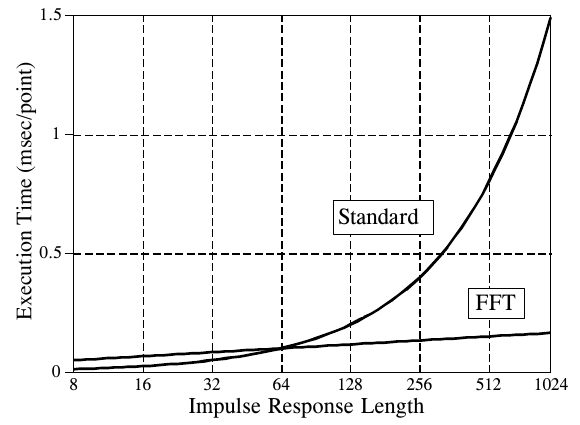
\includegraphics[width=0.483\linewidth,height=0.8\textheight,keepaspectratio]{assets/ch18/fig18-03.png}
\caption*{\textbf{图 18-3　FFT 卷积的执行时间。} 当滤波器核长于约 60 点时，FFT
卷积比标准方法快。这些执行时间是在 100 MHz
奔腾上、使用单精度浮点数测得的。 （Execution Time (msec/point) =
执行时间（毫秒/点），Impulse Response Length = 冲激响应长度；Standard =
标准卷积，FFT = FFT
卷积。原书图注排在图的左边，裁图时已去掉，译文见上。）}
\end{figure}

要记住的要点是：短于约 60
点的滤波器核用标准卷积实现更快，执行时间与核的长度成正比。更长的滤波器核用
FFT 卷积实现更快。用 FFT
卷积时，滤波器核想做多长都可以，执行时间几乎不受影响。例如，一个 16,000
点的滤波器核，执行时间只比 64 点的核长大约一倍。

卷积的速度也决定了计算的精度（就像第 12 章讲 FFT
时说的那样）。这是因为输出信号中的舍入误差取决于计算的总次数，而计算次数与计算时间成正比。输出信号算得越快，也就算得越精确。例如，设想用单精度浮点数把一个信号与一个
1000
点的滤波器核卷积。用标准卷积，典型的舍入噪声预计约为两万分之一（根据第 4
章的经验法则）。相比之下，FFT
卷积预计会快一个数量级，精度也高一个数量级（即二十万分之一）。

把 FFT
卷积收好，留到你有大量数据要处理、又需要极长的滤波器核时再用。想想一百万个采样的信号和一千点的滤波器核这样的规模。达不到这个规模，就不值得多花这些编程功夫。不想自己写
FFT
卷积程序？去软件库和软件包里找现成的代码。可以先从本书的网站找起（见版权页）。
